% !TEX program = xelatex
\documentclass[13pt,a4paper]{extreport}
\usepackage[a4paper,left=2.5cm,right=2cm,top=2.7cm,bottom=2.5cm,headheight=30pt]{geometry}
\usepackage{fontspec}
\setmainfont{TeX Gyre Termes}
\setmonofont{TeX Gyre Cursor}[Scale=0.88]
\usepackage{xcolor,graphicx,booktabs,tabularx,array,float,caption,subcaption,amsmath,amssymb,enumitem,fancyhdr,titlesec,tikz,listings,algorithm,algpseudocode,hyperref,setspace}
\usetikzlibrary{positioning,shapes,arrows.meta}
\hypersetup{colorlinks=true,linkcolor=black,urlcolor=blue,citecolor=black}
\renewcommand{\baselinestretch}{1.2}
\setlength{\parindent}{1cm}\setlength{\parskip}{3pt}
\captionsetup{font=small,labelsep=colon}

% ---------- metadata ----------
\newcommand{\TenMon}{Trí tuệ Nhân tạo Nâng cao}
\newcommand{\TenDeTai}{Xây dựng và Đánh giá Game AI Cờ vua Đa cấp độ}
\newcommand{\GVHD}{Đỗ Như Tài}
\newcommand{\NhomSo}{27}
\newcommand{\RepoURL}{https://github.com/nduc2407/chess-ai-alphazero-mcts}
\newcommand{\CommitNop}{70ac9fa (nhánh feature/tv1-core-search-rl) + thư mục report/}
\newcommand{\NgayThang}{THÁNG 11/2026}

% ---------- tiêu đề ----------
\titleformat{\chapter}[block]{\centering\bfseries\Large}{\MakeUppercase{Chương \thechapter.}}{0.5em}{\MakeUppercase}
\titlespacing*{\chapter}{0pt}{-10pt}{18pt}
\titleformat{\section}{\bfseries\large\sffamily\selectfont}{\thesection}{0.8em}{}
\titleformat{\subsection}{\bfseries\normalsize\sffamily\selectfont}{\thesubsection}{0.8em}{}
\renewcommand{\thetable}{\thechapter.\arabic{table}}
\renewcommand{\thefigure}{\thechapter.\arabic{figure}}
\renewcommand{\tablename}{Bảng}\renewcommand{\figurename}{Hình}
\renewcommand{\contentsname}{Mục lục}
\renewcommand{\listtablename}{Danh sách bảng}\renewcommand{\listfigurename}{Danh sách hình}
\floatname{algorithm}{Thuật toán}
\renewcommand{\algorithmicrequire}{\textbf{Đầu vào:}}\renewcommand{\algorithmicensure}{\textbf{Đầu ra:}}

% ---------- header ----------
\pagestyle{fancy}\fancyhf{}
\fancyhead[L]{\raisebox{-0.45cm}{
\includegraphics[height=1cm]{logo.png}}\hspace{0.5em}\begin{minipage}[b]{8cm}\small Trường Đại học Sài Gòn\\[-2pt]\normalsize Khoa Công nghệ Thông tin\end{minipage}}
\fancyfoot[C]{\thepage}
\renewcommand{\headrulewidth}{0.4pt}
\fancypagestyle{plain}{\fancyhf{}\fancyhead[L]{\raisebox{-0.45cm}{
\includegraphics[height=1cm]{logo.png}}\hspace{0.5em}\begin{minipage}[b]{8cm}\small Trường Đại học Sài Gòn\\[-2pt]\normalsize Khoa Công nghệ Thông tin\end{minipage}}\fancyfoot[C]{\thepage}\renewcommand{\headrulewidth}{0.4pt}}
\newcommand{\chuong}[1]{\chapter*{#1}\addcontentsline{toc}{chapter}{#1}\markboth{}{}}
\newcommand{\tieude}[1]{\begin{center}\bfseries\Large\MakeUppercase{#1}\end{center}\vspace{0.6cm}}

% ---------- code ----------
\lstset{basicstyle=\ttfamily\footnotesize,breaklines=true,frame=tb,backgroundcolor=\color{black!4},columns=fullflexible,keepspaces=true}
\newcommand{\code}[1]{\texttt{#1}}
\newcolumntype{Y}{>{\raggedright\arraybackslash}X}

\begin{document}
% ================= TRANG BÌA =================
\begin{titlepage}
\centering
{\bfseries\large TRƯỜNG ĐẠI HỌC SÀI GÒN\\ KHOA CÔNG NGHỆ THÔNG TIN\par}
\vspace{1cm}

\includegraphics[width=4.2cm]{logo.png}\par
\vspace{1.6cm}
\rule{\textwidth}{0.5pt}\\[0.4cm]
{\bfseries\large \TenMon\par}
\vspace{0.3cm}\rule{\textwidth}{0.5pt}\\[0.5cm]
{\bfseries\fontsize{22}{26}\selectfont \TenDeTai\par}
\vspace{0.3cm}\rule{\textwidth}{0.5pt}
\vspace{2.2cm}

\begin{flushleft}\hspace{3.2cm}
\begin{tabular}{@{}l l l@{}}
\textbf{GVHD:} & \GVHD & \\[4pt]
\textbf{Nhóm \NhomSo:} & Đặng Nhật Đức & 3123410082 \\
 & Võ Văn Tuấn & 3123410414 \\
 & Nguyễn Thái Vinh & 3123410433 \\
\end{tabular}
\end{flushleft}
\vspace{1.6cm}
{\small Báo cáo đồ án cuối kỳ\\
Repo: \texttt{\RepoURL}\\
Commit nộp bài: \CommitNop\par}
\vfill
{\small TP. HỒ CHÍ MINH, \NgayThang\par}
\end{titlepage}

\pagenumbering{roman}
% ================= NHẬN XÉT =================
\chuong{Nhận xét của giảng viên}
\tieude{Nhận xét của giảng viên}
\vspace{-0.3cm}
\foreach \i in {1,...,14}{\noindent\dotfill\par\vspace{0.55cm}}
\vfill
\noindent\textbf{Điểm:} \dotfill\hspace{0.5cm}\hfill\parbox{8cm}{\centering\textit{TP. Hồ Chí Minh, ngày \ldots{} tháng \ldots{} năm 20\ldots}\\ \textbf{Giảng viên}\\ \textit{(Ký và ghi rõ họ tên)}\\[1.8cm] \GVHD}
\clearpage

% ================= LỜI CẢM ƠN =================
\chuong{Lời cảm ơn}
\tieude{Lời cảm ơn}
Nhóm xin chân thành cảm ơn thầy \GVHD{} đã định hướng đề tài, đưa ra yêu cầu rõ ràng về thực nghiệm và liêm chính học thuật, giúp nhóm tập trung vào việc \emph{chứng minh tác dụng của từng thành phần} thay vì chỉ liệt kê thuật toán. Nhóm cũng cảm ơn Khoa Công nghệ Thông tin, Trường Đại học Sài Gòn đã tạo điều kiện học tập, và cộng đồng mã nguồn mở (đặc biệt là thư viện \texttt{python-chess}) đã cung cấp nền tảng luật cờ chuẩn FIDE.

\vspace{1cm}
\begin{flushright}\textit{TP. Hồ Chí Minh, tháng 11/2026}\\ \textbf{Nhóm \NhomSo}\end{flushright}
\clearpage

\tableofcontents\clearpage
\listoftables\clearpage
\listoffigures\clearpage

% ================= VIẾT TẮT =================
\chuong{Danh mục từ viết tắt}
\tieude{Danh mục từ viết tắt}
\begin{tabular}{@{}p{2.2cm}p{11cm}@{}}
\toprule \textbf{Viết tắt} & \textbf{Ý nghĩa}\\ \midrule
AB & Alpha-Beta (cắt tỉa alpha-beta)\\
EPD & Extended Position Description --- định dạng mô tả thế cờ\\
FEN & Forsyth--Edwards Notation\\
ID & Iterative Deepening --- đào sâu dần\\
MCTS & Monte Carlo Tree Search --- tìm kiếm cây Monte Carlo\\
MVV-LVA & Most Valuable Victim -- Least Valuable Attacker\\
PST & Piece-Square Table --- bảng điểm quân--ô\\
PUCT & Predictor + UCT (dùng trong AlphaGo/AlphaZero)\\
RL & Reinforcement Learning --- học tăng cường\\
SAN & Standard Algebraic Notation\\
TT & Transposition Table --- bảng chuyển vị\\
UCT & Upper Confidence bounds applied to Trees\\
WAC & Win At Chess --- bộ 50 thế cờ chiến thuật dùng trong báo cáo\\
\bottomrule\end{tabular}
\clearpage
\pagenumbering{arabic}

% ================= LỜI MỞ ĐẦU =================
\chuong{Lời mở đầu}
\tieude{Lời mở đầu}
Báo cáo này trình bày hệ thống Game AI Cờ vua chuẩn FIDE $8\times 8$ gồm nhiều cấp độ tác tử và kết quả đánh giá thực nghiệm. Báo cáo bám cấu trúc 5 chương theo đề bài: Giới thiệu; Cơ sở lý thuyết; Phương pháp và thiết kế hệ thống; Thực nghiệm, kết quả và thảo luận; Kết luận.

\paragraph{Nguyên tắc trung thực số liệu.} Mọi con số trong Chương 4 được sinh trực tiếp từ log thật do các script trong kho mã chạy ra (\code{scripts/run\_real\_experiments.py}, \code{scripts/analyze\_real\_results.py}; log nằm ở \code{results/} và \code{logs/}). Phạm vi \emph{đã cài đặt và đã chạy} của kho mã tại thời điểm viết báo cáo là \textbf{Cấp 1 đến Cấp 4} (Random, Heuristic, Alpha-Beta, UCT). Các Cấp 5--8 (mạng nơ-ron có giám sát, RL cờ tàn KRK, Guided MCTS, AlphaZero-style) mới có khung giao diện trong mã, chưa được cài đặt và chưa được huấn luyện; vì vậy báo cáo \textbf{không} đưa bất kỳ kết quả huấn luyện, learning curve hay đối đầu nào cho các cấp này, và chỉ mô tả chúng như thiết kế dự kiến (Mục~\ref{sec:future}).

% ================= CHƯƠNG 1 =================
\chapter{Giới thiệu}
\section{Bối cảnh}
Cờ vua là bài toán kinh điển của trí tuệ nhân tạo: trò chơi hai người, thông tin hoàn hảo, tổng bằng không, với hệ số rẽ nhánh trung bình khoảng 30--35 và độ dài ván hàng chục nước. Lịch sử phát triển từ tìm kiếm đối kháng cổ điển (Minimax, Alpha-Beta) \cite{knuth1975}, sang MCTS \cite{kocsis2006}, rồi các hệ thống kết hợp mạng nơ-ron với tìm kiếm như AlphaGo \cite{silver2016} và AlphaZero \cite{silver2017}. Đồ án xây dựng một chuỗi tác tử tăng dần độ phức tạp trên cùng một môi trường để đo \emph{đóng góp thực sự của từng thành phần}.

\section{Game, luật và ý nghĩa}
Trò chơi là cờ vua FIDE đầy đủ trên bàn $8\times 8$ (nhập thành, bắt tốt qua đường, phong cấp, chiếu hết, hòa bí nước, thiếu lực lượng, lặp thế ba lần, luật 50 nước). Luật được ủy thác cho thư viện \code{python-chess} thông qua lớp bọc \code{ChessEnv}; nhóm không tự cài lại bộ sinh nước đi. Ý nghĩa: cờ vua đủ phức tạp để các kỹ thuật tìm kiếm có sự khác biệt rõ rệt, nhưng vẫn có thể đánh giá trên máy cá nhân với ngân sách nhỏ.

\section{Mục tiêu và câu hỏi nghiên cứu}
\textbf{Mục tiêu:} xây dựng môi trường cờ vua, các tác tử tìm kiếm cổ điển, và quy trình giải đấu công bằng để so sánh chúng. Các câu hỏi nghiên cứu:
\begin{enumerate}[label=\textbf{RQ\arabic*.},leftmargin=1.6cm]
\item Mỗi thành phần của Alpha-Beta (cắt tỉa, sắp xếp nước đi, bảng chuyển vị, tìm kiếm tĩnh) đóng góp bao nhiêu vào số nút duyệt và độ chính xác chiến thuật?
\item Với ngân sách tính toán cố định, xếp hạng của Random, Heuristic, Alpha-Beta và UCT là gì?
\item UCT thuần (rollout ngẫu nhiên có cắt ngưỡng) cần bao nhiêu mô phỏng để thắng tác tử Heuristic một nước đi?
\item (Chưa trả lời được) Mạng chính sách/giá trị và tự chơi cải thiện sức chơi bao nhiêu so với tìm kiếm cổ điển? Câu hỏi này cần Cấp 5--8, chưa được thực hiện.
\end{enumerate}

\section{Phạm vi}
\begin{itemize}
\item Đã thực hiện: môi trường + kiểm thử, Cấp 1--4, giải đấu vòng tròn, hai ablation, benchmark WAC-50.
\item Chưa thực hiện: Cấp 5--8, ETL dữ liệu Lichess, huấn luyện, giao diện Pygame, module arena chính thức (các file này là khung chưa cài đặt trong repo; giải đấu trong báo cáo dùng script riêng ghi ở Mục~\ref{sec:fair}).
\item Chế độ ngân sách: chỉ \emph{workload-control} (số nút/số mô phỏng cố định); chế độ time-control chưa chạy.
\end{itemize}

\section{Sản phẩm}
Kho mã \texttt{\RepoURL} gồm package \code{chess\_ai/} (môi trường, tìm kiếm, tác tử), cấu hình YAML, bộ kiểm thử \code{pytest}, và (do nhóm bổ sung trong đợt viết báo cáo) thư mục \code{scripts/}, \code{results/}, \code{logs/}, \code{report/}. Mã báo cáo LaTeX nằm trong \code{report/}.

% ================= CHƯƠNG 2 =================
\chapter{Cơ sở lý thuyết và công trình liên quan}
\section{Tác tử trò chơi}
Tác tử nhận trạng thái $s$ và chọn hành động $a\in\mathcal A(s)$. Với trò chơi tổng bằng không, hai người, thông tin hoàn hảo, giá trị trạng thái thỏa phương trình Minimax; hàm lượng giá tĩnh $h(s)$ thay cho giá trị thật khi cắt độ sâu \cite{russell2021}.

\section{Minimax, Alpha-Beta}
Dạng Negamax: $V(s,d)=\max_a\,-V(s',d-1)$, $V(s,0)=h(s)$. Cắt tỉa Alpha-Beta duy trì cửa sổ $[\alpha,\beta]$ và bỏ nhánh khi $\alpha\ge\beta$, cho cùng kết quả như Minimax nhưng duyệt ít nút hơn nhiều khi thứ tự nước đi tốt \cite{knuth1975}. Các cải tiến chuẩn: đào sâu dần (ID), sắp xếp nước đi (nước từ TT, MVV-LVA, killer, history), bảng chuyển vị khóa Zobrist, và tìm kiếm tĩnh (quiescence) để giảm hiệu ứng chân trời.

\section{MCTS và UCT}
MCTS lặp bốn bước: chọn, mở rộng, mô phỏng, lan truyền ngược. UCT chọn nút con theo
\begin{equation}
a^*=\arg\max_a\Big(\frac{W(s,a)}{N(s,a)}+c\sqrt{\frac{\ln N(s)}{N(s,a)}}\Big),\quad c=\sqrt2,
\end{equation}
\cite{kocsis2006}. Ưu điểm: không cần hàm lượng giá; nhược điểm: với hệ số rẽ nhánh lớn và rollout ngẫu nhiên, ước lượng giá trị nhiễu khi ngân sách mô phỏng nhỏ.

\section{Mạng chính sách/giá trị, RL và tự chơi}
AlphaGo dùng mạng chính sách $p(a|s)$ huấn luyện có giám sát rồi tinh chỉnh bằng RL, cùng mạng giá trị $v(s)$, kết hợp trong MCTS \cite{silver2016}. AlphaZero bỏ dữ liệu người, dùng một mạng hai đầu $(p,v)$ và chọn nút bằng PUCT:
\begin{equation}
a^*=\arg\max_a\Big(Q(s,a)+c_{\text{puct}}\,P(s,a)\frac{\sqrt{N(s)}}{1+N(s,a)}\Big),
\end{equation}
huấn luyện hoàn toàn bằng tự chơi \cite{silver2017}. Khái niệm MDP và RL xem \cite{sutton2018}.

\section{Phân biệt AlphaGo-inspired và AlphaZero-inspired}
\emph{AlphaGo-inspired}: mạng huấn luyện có giám sát trên ván người + tìm kiếm có dẫn đường. \emph{AlphaZero-inspired}: vòng lặp tự chơi $\to$ huấn luyện $\to$ kiểm định (gating) không dùng dữ liệu người. Trong đồ án, hai hướng này chỉ ở mức thiết kế (Mục~\ref{sec:future}); không có kết quả thực nghiệm nào được báo cáo cho chúng.

% ================= CHƯƠNG 3 =================
\chapter{Phương pháp và thiết kế hệ thống}
\section{Biểu diễn game, state, action, reward}
\begin{itemize}
\item \textbf{State:} đối tượng \code{chess.Board} (bitboard) gồm vị trí quân, lượt đi, quyền nhập thành, ô bắt tốt qua đường, bộ đếm nửa nước, lịch sử lặp thế.
\item \textbf{Action:} nước đi hợp lệ \code{chess.Move} từ \code{legal\_actions()}.
\item \textbf{Reward:} phần thưởng cuối ván $+1/0/-1$ theo góc nhìn bên vừa đi; không có phần thưởng trung gian.
\item \textbf{Kết thúc:} chiếu hết, hòa bí, thiếu lực lượng, lặp thế ba lần, luật 50 nước (\code{is\_game\_over(claim\_draw=True)}).
\end{itemize}

\section{Kiến trúc hệ thống}
\begin{figure}[H]\centering
\begin{tikzpicture}[khoi/.style={draw,rounded corners,fill=blue!8,minimum width=2.5cm,minimum height=1cm,align=center,font=\small},mui/.style={-Stealth,thick},node distance=0.9cm]
\node[khoi] (env) {\code{ChessEnv}\\luật + state};
\node[khoi,right=of env] (ag) {\code{BaseAgent}\\\code{select\_move}};
\node[khoi,right=of ag] (se) {Tìm kiếm\\AB / UCT};
\node[khoi,below=of ag,fill=green!10] (ar) {Giải đấu\\(script thực nghiệm)};
\node[khoi,right=of ar,fill=green!10] (log) {Log \code{jsonl}\\+ phân tích};
\draw[mui] (env)--(ag);\draw[mui] (ag)--(se);\draw[mui] (ar)--(ag);\draw[mui] (ar)--(log);
\end{tikzpicture}
\caption{Kiến trúc: môi trường, tác tử, tìm kiếm và quy trình giải đấu/ghi log.}\end{figure}
Giao diện chung \code{BaseAgent.select\_move(env, time\_limit, max\_workload)} cho phép mọi tác tử dùng cùng ngân sách. Hàm lượng giá (\code{evaluation.py}) gồm vật chất, bảng PST kiểu Michniewski (có hai bảng Vua trung/tàn cuộc) và điểm an toàn Vua, trả về centipawn theo góc nhìn bên đi.

\section{Thuật toán từng cấp}
\paragraph{Cấp 1 --- Random.} Chọn đều ngẫu nhiên trong các nước hợp lệ (có seed).
\paragraph{Cấp 2 --- Heuristic một nước.} Theo thứ tự: (i) chiếu hết ngay nếu có; (ii) loại nước để đối thủ chiếu hết ngay; (iii) với mỗi nước còn lại tính lượng giá tĩnh sau nước đi, trừ $0{,}85\times$ mức thiệt hại bắt quân lớn nhất mà đối thủ có thể gây ra (xấp xỉ SEE), và phạt lặp thế khi đang hơn.
\paragraph{Cấp 3 --- Alpha-Beta.} Negamax + ID, sắp xếp nước (PV từ TT, MVV-LVA, killer, history), TT Zobrist, quiescence; dừng theo số nút hoặc thời gian.
\begin{algorithm}[H]\caption{Negamax Alpha-Beta (rút gọn)}
\begin{algorithmic}[1]
\Function{Search}{$s,d,\alpha,\beta$}
\If{$d=0$} \State \Return \Call{Quiescence}{$s,\alpha,\beta$} \EndIf
\State tra TT; sắp xếp nước đi
\For{$a$ trong các nước đã sắp xếp}
 \State $v\gets -\Call{Search}{s\!\cdot\!a,d-1,-\beta,-\alpha}$
 \State $\alpha\gets\max(\alpha,v)$;\ \textbf{if} $\alpha\ge\beta$ \textbf{then} \textbf{break}
\EndFor
\State lưu TT; \Return $\alpha$
\EndFunction
\end{algorithmic}\end{algorithm}
\paragraph{Cấp 4 --- UCT thuần.} UCB1 với $c=1{,}414$; mô phỏng ngẫu nhiên tối đa 60 plies, trong rollout bắt quân được ưu tiên với xác suất 0,7; nếu chưa kết thúc, giá trị lá là $\tanh(h(s)/600)$; có tái sử dụng cây con.

\section{Dữ liệu và quy trình huấn luyện}
Các Cấp 1--4 \textbf{không dùng dữ liệu huấn luyện}. Do đó không có quy trình train, loss hay checkpoint nào được báo cáo. Dữ liệu duy nhất là: (i) bộ WAC-50 (\code{resources/benchmark\_positions.epd}, 50 thế chiến thuật \cite{reinfeld1982}) và (ii) bộ khai cuộc sinh tự động ở Mục~\ref{sec:fair}.

\section{Thiết kế giải đấu công bằng}\label{sec:fair}
\begin{itemize}
\item \textbf{Khai cuộc:} tệp \code{resources/openings\_50.epd} trong repo chỉ có phần chú thích (không có thế cờ nào), nên nhóm sinh 50 thế bằng script: 8 plies ngẫu nhiên (seed $=2024$), giữ thế có $|h|\le 60$ cp, loại trùng; lưu ở \code{results/round\_robin/openings\_generated.epd}. Giải đấu dùng 16 thế đầu.
\item \textbf{Cân bằng lượt:} mỗi cặp đấu mỗi thế hai ván, đổi màu $\Rightarrow$ 32 ván/cặp.
\item \textbf{Ngân sách (workload-control):} Cấp 3: 2000 nút/nước; Cấp 4: 200 mô phỏng/nước; Cấp 1, 2 không có tham số ngân sách.
\item \textbf{Giới hạn:} 300 plies; vượt giới hạn tính hòa (được ghi riêng là \code{max\_plies}).
\item \textbf{Seed:} Cấp 1, 2, 4 dùng seed $1000+i$ theo chỉ số khai cuộc; Cấp 3 tất định.
\item \textbf{Độ đo:} thắng/hòa/thua, điểm $=(W+0{,}5D)/N$, khoảng tin cậy Wilson 95\% và bootstrap 10\,000 lần theo khai cuộc (mỗi khai cuộc gồm hai ván đổi màu), độ trễ mỗi nước, số nút/mô phỏng.
\end{itemize}

% ================= CHƯƠNG 4 =================
\chapter{Thực nghiệm, kết quả và thảo luận}
\section{Môi trường chạy}
Máy ảo Linux 2 nhân CPU, không GPU; Python 3.13, \code{python-chess} 1.11.2; mã tại commit \code{70ac9fa}. Hai tiến trình song song chạy các ván; độ trễ đo bằng \code{time.perf\_counter} nên có thể bị ảnh hưởng nhẹ do chia sẻ CPU. Bộ kiểm thử có sẵn của repo (\code{pytest}) cho \textbf{11 test đạt}, gồm: luật cơ bản, nước bất hợp lệ và chiếu hết, đối xứng lượng giá, TT, Alpha-Beta duyệt ít nút hơn Minimax, các tác tử trả nước hợp lệ, chiếu hết một nước ở Cấp 2--4, tái sử dụng cây con của UCT. Quy mô thực nghiệm: 192 ván giải đấu, 96 ván ablation UCT, 50 thế WAC cho 6 cấu hình, 10 cấu hình ablation tìm kiếm.

\section{Ma trận đối đầu và thắng/hòa/thua}
\begin{table}[H]\centering\small
\caption{Kết quả vòng tròn (workload-control). W/D/L tính theo tác tử đứng đầu cặp. Điểm $=(W+0{,}5D)/N$.}\label{tab:pairs}\footnotesize\setlength{\tabcolsep}{3pt}
\begin{tabular}{l r c c c c r r}
\toprule
Cặp & $N$ & W/D/L (A) & Điểm A & Wilson 95\% & Bootstrap 95\% & Hòa cap & Plies TB \\
\midrule
Cấp 1 -- Cấp 2 & 32 & 0 / 0 / 32 & 0,000 & {[0,000; 0,107]} & {[0,000; 0,000]} & 0 & 36,6 \\
Cấp 1 -- Cấp 3 & 32 & 0 / 0 / 32 & 0,000 & {[0,000; 0,107]} & {[0,000; 0,000]} & 0 & 33,9 \\
Cấp 1 -- Cấp 4 & 32 & 0 / 7 / 25 & 0,109 & {[0,041; 0,262]} & {[0,047; 0,188]} & 7 & 141,9 \\
Cấp 2 -- Cấp 3 & 32 & 0 / 8 / 24 & 0,125 & {[0,050; 0,281]} & {[0,062; 0,188]} & 0 & 81,4 \\
Cấp 2 -- Cấp 4 & 32 & 32 / 0 / 0 & 1,000 & {[0,893; 1,000]} & {[1,000; 1,000]} & 0 & 37,8 \\
Cấp 3 -- Cấp 4 & 32 & 32 / 0 / 0 & 1,000 & {[0,893; 1,000]} & {[1,000; 1,000]} & 0 & 30,6 \\
\bottomrule
\end{tabular}
\end{table}
\begin{figure}[H]\centering
\begin{subfigure}{0.48\textwidth}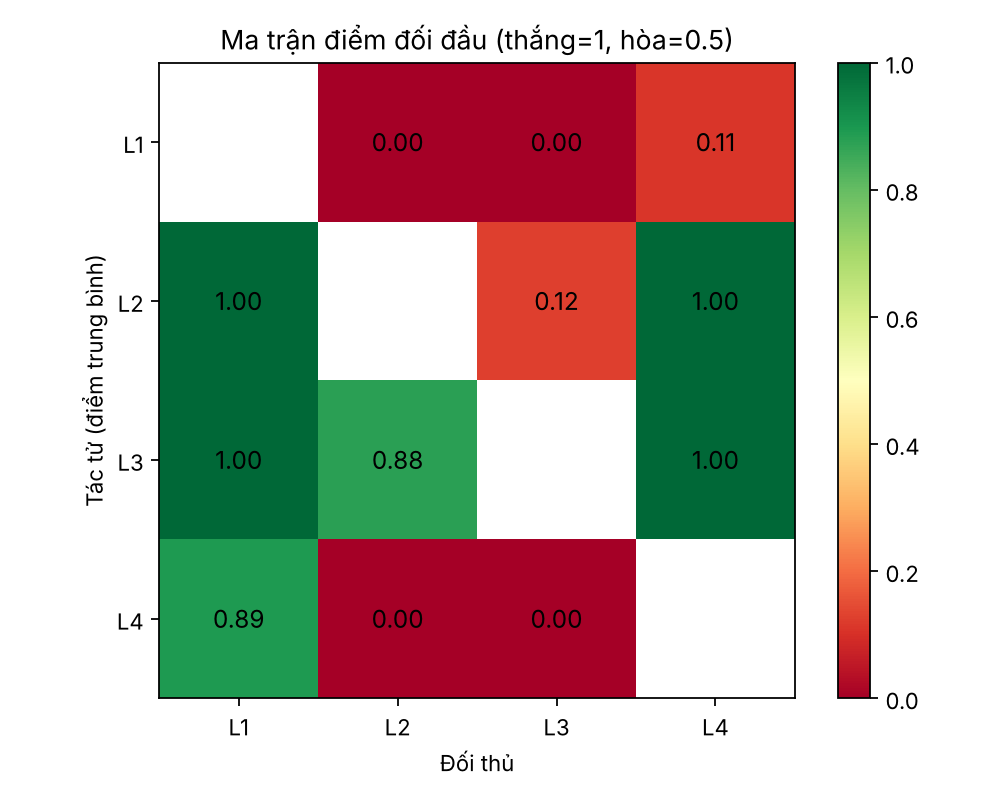
\includegraphics[width=\textwidth]{figures/matrix_score.png}\caption{Ma trận điểm.}\end{subfigure}\hfill
\begin{subfigure}{0.5\textwidth}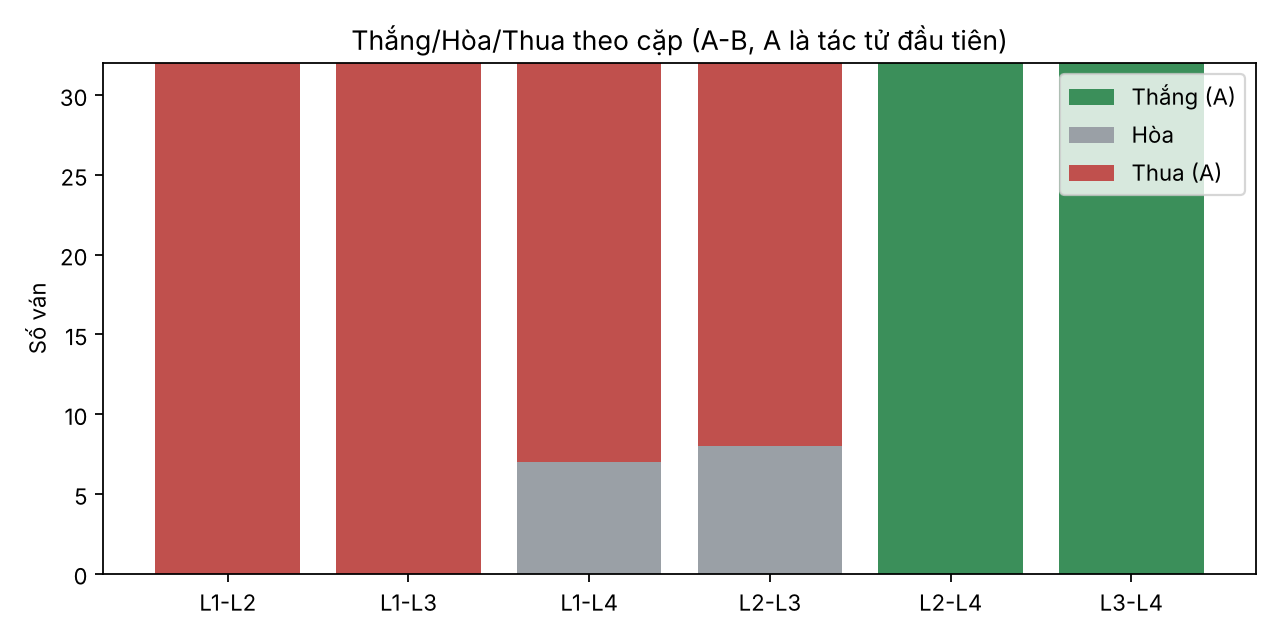
\includegraphics[width=\textwidth]{figures/wdl_pairs.png}\caption{Thắng/hòa/thua theo cặp.}\end{subfigure}
\caption{Kết quả giải đấu vòng tròn Cấp 1--4 (sinh từ \code{scripts/analyze\_real\_results.py}).}\label{fig:matrix}\end{figure}
Thứ hạng quan sát được: \textbf{Cấp 3 $>$ Cấp 2 $>$ Cấp 4 $>$ Cấp 1} theo điểm trung bình toàn giải (96 ván mỗi tác tử): Cấp 3 đạt 0,958; Cấp 2 đạt 0,708; Cấp 4 đạt 0,297; Cấp 1 đạt 0,036 (Bảng~\ref{tab:lat}). Điểm lưu ý: ở các cặp có kết quả 0--32 hoặc 32--0, khoảng bootstrap suy biến thành một điểm vì mọi khai cuộc cho cùng kết quả; khi đó khoảng Wilson (cận trên 0,107 hay cận dưới 0,893) là chỉ báo thận trọng hơn.

\section{Độ trễ và chi phí}
\begin{table}[H]\centering\small
\caption{Độ trễ mỗi nước (ms) và khối lượng tìm kiếm trung bình mỗi nước. Cấp 3 tính nút; Cấp 4 tính mô phỏng; Cấp 2 tính số nước ứng viên.}\label{tab:lat}
\begin{tabular}{l r r r r}
\toprule
Tác tử & Trễ TB & Trễ tối đa & Nút/mô phỏng TB & Điểm toàn giải \\
\midrule
Cấp 1 & 0,03 & 0,1 & 1,0 & 0,036 \\
Cấp 2 & 5,91 & 19,2 & 31,5 & 0,708 \\
Cấp 3 & 68,14 & 134,5 & 1906,6 & 0,958 \\
Cấp 4 & 469,33 & 630,8 & 200,0 & 0,297 \\
\bottomrule
\end{tabular}
\end{table}
Cấp 3 với 2000 nút (khoảng 68 ms/nước) thắng Cấp 4 với 200 mô phỏng (khoảng 469 ms/nước) tuyệt đối dù dùng thời gian ít hơn khoảng 7 lần, nên so sánh theo thời gian thực chỉ làm khoảng cách lớn hơn; tuy nhiên chế độ time-control chưa được chạy nên không có số liệu trực tiếp.

\section{Ablation 1: các thành phần của Alpha-Beta}
Trên 50 thế WAC-50, cố định độ sâu tối đa $d\in\{2,3\}$ (ID), thêm dần từng thành phần. ``Giải đúng'' nghĩa là nước chọn nằm trong tập \code{bm} của thế.
\begin{table}[H]\centering\small
\caption{Ablation Alpha-Beta trên WAC-50. Nút TB là số nút trung bình mỗi thế; hệ số giảm tính so với Minimax thuần cùng độ sâu.}\label{tab:abs}
\begin{tabular}{c l r r r r}
\toprule
$d$ & Cấu hình & Nút TB & Giảm & Tổng thời gian (s) & Giải đúng \\
\midrule
2 & Minimax thuần & 1345 & 1,0$\times$ & 3,05 & 11/50 \\
2 & + Alpha-Beta & 540 & 2,5$\times$ & 1,27 & 11/50 \\
2 & + Move Ordering & 192 & 7,0$\times$ & 0,54 & 11/50 \\
2 & + TT & 191 & 7,0$\times$ & 0,48 & 11/50 \\
2 & + Quiescence (đầy đủ) & 1116 & 1,2$\times$ & 2,33 & 26/50 \\
3 & Minimax thuần & 51495 & 1,0$\times$ & 115,97 & 27/50 \\
3 & + Alpha-Beta & 7246 & 7,1$\times$ & 15,92 & 27/50 \\
3 & + Move Ordering & 2016 & 25,5$\times$ & 4,70 & 27/50 \\
3 & + TT & 1962 & 26,3$\times$ & 4,51 & 27/50 \\
3 & + Quiescence (đầy đủ) & 4704 & 10,9$\times$ & 7,68 & 37/50 \\
\bottomrule
\end{tabular}
\end{table}
\begin{figure}[H]\centering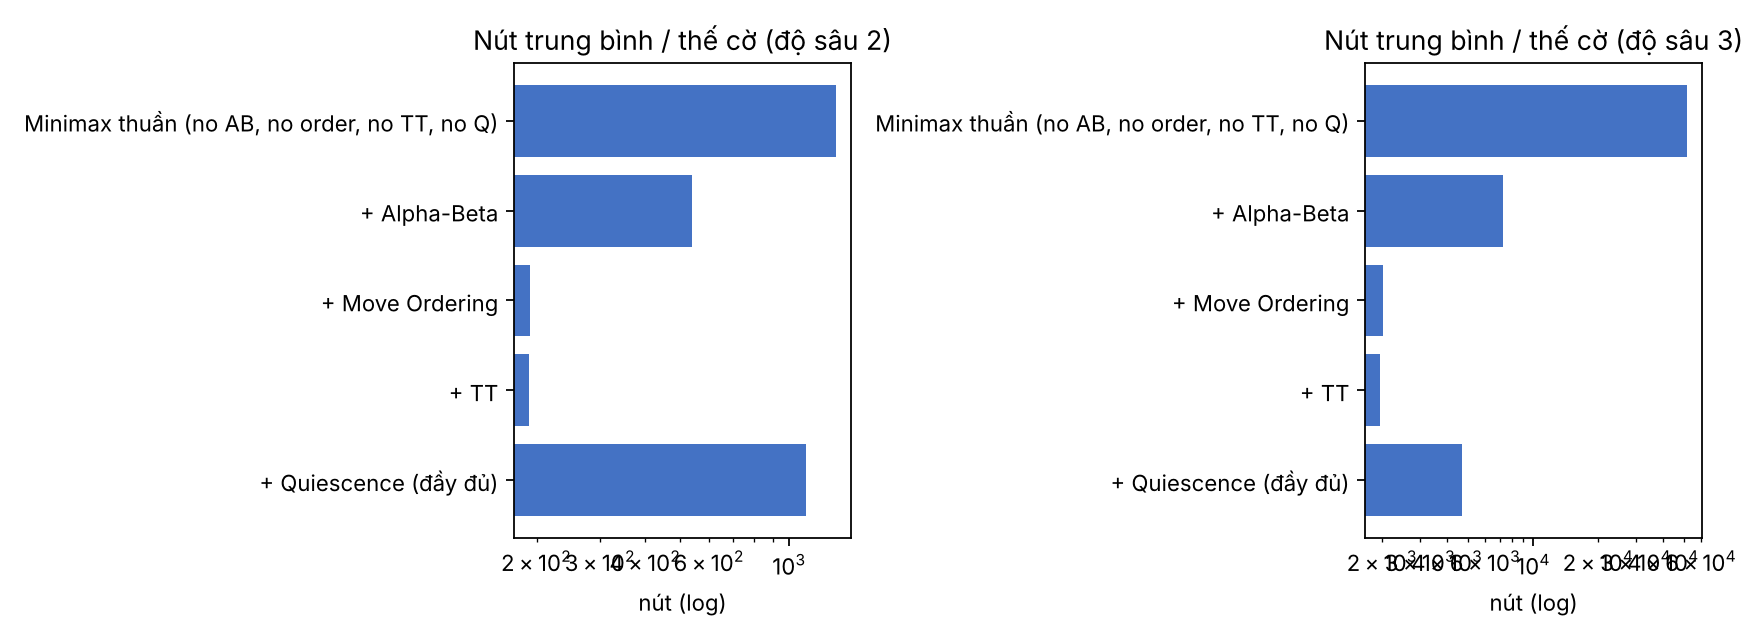
\includegraphics[width=0.95\textwidth]{figures/ablation_search_nodes.png}\caption{Số nút trung bình theo cấu hình (thang log).}\end{figure}
\textbf{Nhận xét (đo được):} (i) Alpha-Beta giảm số nút khoảng 7,1 lần ở $d=3$ mà không đổi kết quả (27/50 trước và sau), phù hợp với tính chất đảm bảo cùng giá trị Minimax. (ii) Sắp xếp nước đi giảm thêm khoảng 3,6 lần (7246 $\to$ 2016 nút). (iii) TT chỉ giảm thêm khoảng 2,7\% (2016 $\to$ 1962) trong thiết lập này; ở mức độ sâu thấp, ít chuyển vị nên lợi ích nhỏ. (iv) Quiescence \emph{tăng} số nút (khoảng 2,4 lần ở $d=3$) nhưng nâng số thế giải đúng từ 11 lên 26 ($d=2$) và từ 27 lên 37 ($d=3$); đây là thành phần duy nhất làm thay đổi chất lượng nước đi. Tất cả các số trên đến từ một lần chạy với seed cố định; chưa lặp nhiều lần để có độ lệch chuẩn (với tìm kiếm tất định, số nút lặp lại như nhau).

\section{Benchmark chiến thuật WAC-50}
\begin{table}[H]\centering\small
\caption{Số thế WAC-50 chọn đúng nước tốt nhất (mỗi thế một lần, seed 42).}\label{tab:wac}
\begin{tabular}{l l r r}
\toprule
Tác tử & Ngân sách & Giải đúng & Trễ TB (ms) \\
\midrule
Cấp 1 & ---  & 2/50 & 0,03 \\
Cấp 2 & ---  & 5/50 & 8,23 \\
Cấp 3 & 2000 nút & 29/50 & 71,98 \\
Cấp 3 & 10000 nút & 36/50 & 312,61 \\
Cấp 4 & 200 mô phỏng & 3/50 & 391,92 \\
Cấp 4 & 800 mô phỏng & 4/50 & 1600,46 \\
\bottomrule
\end{tabular}
\end{table}
\begin{figure}[H]\centering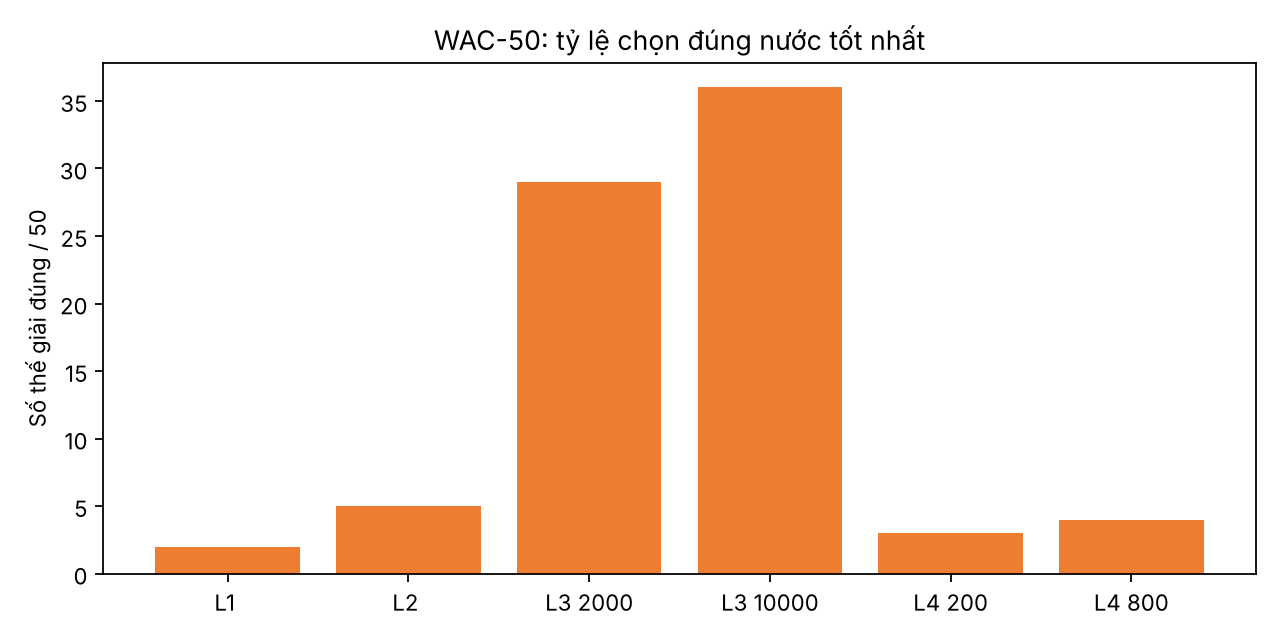
\includegraphics[width=0.6\textwidth]{figures/wac_solved.png}\caption{Số thế WAC giải đúng.}\end{figure}
Cấp 3 giải 29/50 ở 2000 nút và 36/50 ở 10\,000 nút; Cấp 4 chỉ giải 3/50 (200 mô phỏng) và 4/50 (800 mô phỏng); Cấp 1 giải 2/50, tương đương mức đoán ngẫu nhiên thấp. Tăng mô phỏng gấp bốn lần chỉ cải thiện 1 thế, trong khi thời gian tăng khoảng bốn lần.

\section{Ablation 2: số mô phỏng của UCT}
UCT với $\{25,50,100,200\}$ mô phỏng đối đầu Cấp 2, 12 khai cuộc $\times$ 2 màu $=24$ ván mỗi mức.
\begin{table}[H]\centering\small
\caption{UCT (A) đối đầu Cấp 2 theo số mô phỏng.}\label{tab:abm}
\begin{tabular}{r r c c c r}
\toprule
Mô phỏng & $N$ & W/D/L (UCT) & Điểm & Wilson 95\% & Plies TB \\
\midrule
25 & 24 & 0 / 0 / 24 & 0,000 & {[0,000; 0,138]} & 40,5 \\
50 & 24 & 0 / 0 / 24 & 0,000 & {[0,000; 0,138]} & 42,6 \\
100 & 24 & 0 / 0 / 24 & 0,000 & {[0,000; 0,138]} & 39,9 \\
200 & 24 & 0 / 0 / 24 & 0,000 & {[0,000; 0,138]} & 38,8 \\
\bottomrule
\end{tabular}
\end{table}
\begin{figure}[H]\centering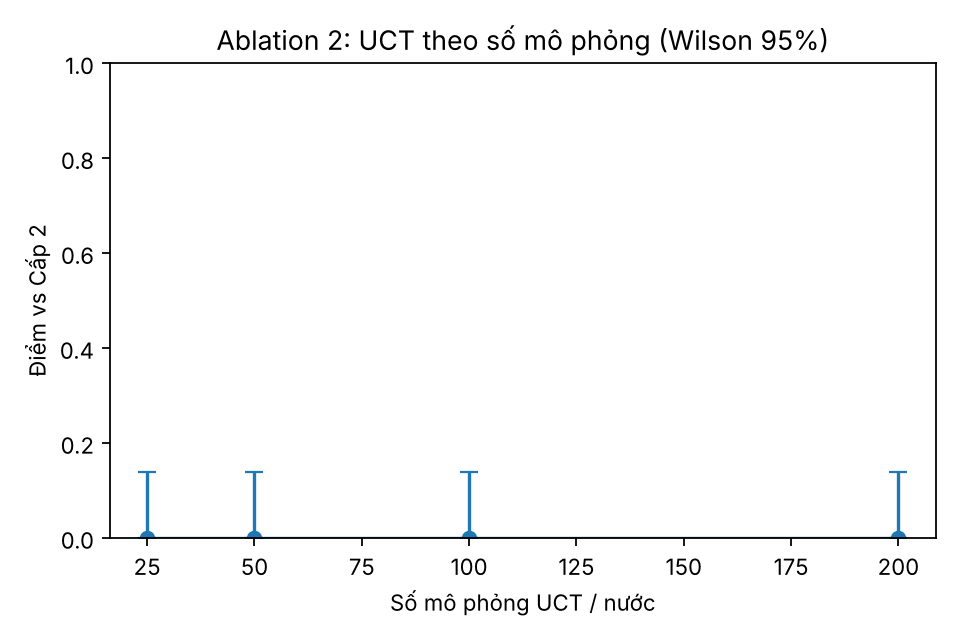
\includegraphics[width=0.55\textwidth]{figures/ablation_mcts.png}\caption{Điểm của UCT so với Cấp 2.}\end{figure}
\textbf{Kết quả:} UCT thua toàn bộ 96 ván ở cả bốn mức, nên trong khoảng 25--200 mô phỏng \emph{không quan sát được xu hướng cải thiện}; trả lời RQ3: với $\le 200$ mô phỏng, UCT thuần không thắng Cấp 2 ván nào. Chưa thử $>200$ mô phỏng trong ván đấu (WAC có thử 800 mô phỏng nhưng không phải ván), nên không thể nói số mô phỏng đủ lớn là bao nhiêu.

\section{Minh họa ván cờ}
Để tránh chọn ván có lợi, quy tắc chọn là cố định trước: khai cuộc đầu tiên trong \code{openings\_generated.epd}, tác tử đứng đầu cặp cầm Trắng. Thế xuất phát (FEN): \texttt{rnb1kbnr/pp1ppp1p/6p1/2p5/q3PP1P/8/PPPPB1P1/RNBQK1NR w KQkq - 1 5
}.
\begin{quote}\footnotesize\textbf{Ván 1.} Trắng: Cấp 3, Đen: Cấp 4; kết quả (góc nhìn Cấp 3): win, 41 plies.\\
5. Nc3 Na6 6. Nxa4 c4 7. Bxc4 f6 8. Nf3 h5 9. Nc3 e5 10. fxe5 Bg7 11. d4 Ne7 12. Be3 fxe5 13. Nxe5 Bxe5 14. dxe5 Nc7 15. O-O Ncd5 16. Nxd5 Nxd5 17. Qxd5 g5 18. Qf7+ Kd8 19. Qf6+ Kc7 20. Qxh8 gxh4 21. Qxh5 d5 22. Bxd5 h3 23. Rf7+ Kb8 24. Qh8 a5 25. Rxb7\#
\end{quote}
\begin{quote}\footnotesize\textbf{Ván 2.} Trắng: Cấp 2, Đen: Cấp 3; kết quả (góc nhìn Cấp 2): draw, 85 plies.\\
5. Nc3 Qd4 6. Nf3 Qd6 7. d4 Nc6 8. Ne5 cxd4 9. Nxc6 dxc6 10. Na4 Nf6 11. Qd3 Qb4+ 12. Nc3 dxc3 13. bxc3 Qxe4 14. Qxe4 Nxe4 15. Bb2 Bg7 16. O-O Bf6 17. h5 Ng3 18. Rfe1 Nxe2+ 19. Rxe2 Bg4 20. Ree1 gxh5 21. Kf2 O-O 22. Rab1 Bf5 23. Re2 e6 24. c4 Bxb2 25. Rxb2 Rab8 26. Re1 Rfd8 27. c5 Rd2+ 28. Kf3 Bxc2 29. Rb4 Bf5 30. a3 h4 31. Rb3 Rc2 32. Re5 f6 33. Rxf5 exf5 34. Rb1 Rc3+ 35. Kf2 Rc2+ 36. Ke3 Rxg2 37. Rd1 Rg3+ 38. Kd4 Rd8+ 39. Kc4 Rxd1 40. a4 Rf1 41. Kb4 Rxf4+ 42. Ka5 Rf2 43. Kb4 Kf8 44. Ka5 Kf7 45. Kb4 Kf8 46. Ka5 Rc2 47. Kb4
\end{quote}
Hai ván này chỉ là minh họa định tính; kết luận định lượng chỉ dựa vào Bảng~\ref{tab:pairs}.

\section{Phân tích thất bại và thảo luận}
\begin{itemize}
\item \textbf{Cấp 4 yếu bất thường:} thua 56/56 ván trước Cấp 2 và Cấp 3 (32 + 24 ván ở ablation). Kiểm tra nhanh cho thấy Cấp 4 tìm được chiếu hết một nước trong các thế thử nên không hỏng hoàn toàn, nhưng trong ván nó mất quân sớm. Giải thích khả dĩ (\emph{giả thuyết, chưa kiểm chứng bằng thực nghiệm riêng}): hệ số rẽ nhánh khoảng 30 với chỉ 200 mô phỏng khiến mỗi nước gốc nhận ít hơn 10 lượt thăm; rollout ngẫu nhiên nhiễu; Cấp 2 và Cấp 3 có kiểm tra thế bị chiếu hết/treo quân tường minh nên không mắc các sai lầm chiến thuật một nước.
\item \textbf{Cấp 4 không mat được Random:} 7/32 ván Cấp 1--Cấp 4 hòa do chạm 300 plies, nghĩa là UCT thuần thắng chậm và không ổn định ở tàn cuộc dù áp đảo vật chất; xu hướng kết ván này không được kiểm tra thêm.
\item \textbf{Cấp 2 vs Cấp 3:} Cấp 3 không thua ván nào (24 thắng, 8 hòa), điểm Cấp 3 $=0{,}875$.
\item \textbf{Mức độ tin cậy:} 32 ván/cặp là nhỏ (đề bài gợi ý 100). Với kết quả cực đoan khoảng tin cậy vẫn rộng (ví dụ 32--0 có cận dưới Wilson 0,893). Cấp 2, 3 tất định nên ván lặp lại nếu cùng khai cuộc và đối thủ; tính độc lập chỉ đến từ khai cuộc khác nhau.
\item \textbf{Ngoại suy:} mọi kết luận chỉ áp dụng cho cờ vua với cấu hình trên; việc suy ra cho trò chơi khác hay cho tác tử học sâu chỉ là giả thuyết.
\end{itemize}

\section{Những thứ chưa có (không báo cáo kết quả)}
Không có learning curve, không có ablation của mạng nơ-ron hay PUCT, không có đối đầu với Cấp 5--8, không có demo giao diện, vì các thành phần này chưa được cài đặt/huấn luyện trong kho mã.

% ================= CHƯƠNG 5 =================
\chapter{Kết luận và hướng phát triển}
\section{Trả lời câu hỏi nghiên cứu}
\begin{itemize}
\item \textbf{RQ1:} Alpha-Beta thuần túy giảm nút khoảng $7\times$ ($d=3$); sắp xếp nước đi giảm thêm khoảng $3{,}6\times$; TT đóng góp nhỏ (khoảng 2,7\%); quiescence làm tăng nút nhưng cải thiện rõ độ chính xác chiến thuật (27 $\to$ 37/50 ở $d=3$).
\item \textbf{RQ2:} Trong thiết lập đã chạy: Cấp 3 $>$ Cấp 2 $>$ Cấp 4 $>$ Cấp 1.
\item \textbf{RQ3:} Với $\le 200$ mô phỏng, UCT thuần không thắng Cấp 2 ván nào trong 96 ván.
\item \textbf{RQ4:} Chưa trả lời, do chưa cài đặt Cấp 5--8.
\end{itemize}
\section{Thành tựu và hạn chế}
\textbf{Thành tựu:} môi trường cờ vua đầy đủ luật có kiểm thử, bốn tác tử, quy trình đánh giá cân bằng màu có log và script tái lập. \textbf{Hạn chế:} mới 4/8 cấp; chưa có thành phần học; chỉ 32 ván/cặp; chưa chạy time-control; bộ khai cuộc sinh tự động thay cho bộ có sẵn trong repo (rỗng); UCT chưa khảo sát với số mô phỏng lớn.

\section{Khả năng tái lập}
Lệnh tái lập (từ gốc repo, cần \code{python-chess}, \code{pyyaml}, \code{numpy}, \code{matplotlib}, \code{scipy}):
\begin{lstlisting}[language=bash]
python3 scripts/run_real_experiments.py openings --n 50
python3 scripts/run_real_experiments.py roundrobin --n 16
python3 scripts/run_real_experiments.py ablation_mcts --n 12
python3 scripts/run_real_experiments.py ablation_search
python3 scripts/run_real_experiments.py wac
python3 scripts/analyze_real_results.py
python3 report/gen_tables.py && cd report && latexmk -xelatex main.tex
\end{lstlisting}
Log thô: \code{results/round\_robin/matches.jsonl}, \code{results/ablation2/matches.jsonl}, \code{results/ablation1/*.json}, \code{results/summary.json}.

\section{Hướng phát triển}\label{sec:future}
Cài đặt Cấp 5 (mạng hai đầu có giám sát, đầu vào 18 kênh $8\times8$), Cấp 7 (PUCT dùng prior/giá trị của Cấp 5) và Cấp 8 (tự chơi + gating), sau đó chạy lại đúng quy trình giải đấu này với 100 ván/cặp và time-control để trả lời RQ4; khảo sát UCT với số mô phỏng lớn hơn và rollout có hướng dẫn. Mọi kết quả dự kiến phải được chạy thật trước khi đưa vào báo cáo.

% ================= TÀI LIỆU THAM KHẢO =================
\chuong{Tài liệu tham khảo}
\tieude{Tài liệu tham khảo}
\begin{thebibliography}{99}\small
\bibitem{knuth1975} Donald E. Knuth and Ronald W. Moore. ``An Analysis of Alpha-Beta Pruning''. In: \emph{Artificial Intelligence} 6.4 (1975), pp. 293--326.
\bibitem{kocsis2006} Levente Kocsis and Csaba Szepesvári. ``Bandit Based Monte-Carlo Planning''. In: \emph{ECML}. 2006, pp. 282--293.
\bibitem{silver2016} David Silver, Aja Huang, Chris J. Maddison, et al. ``Mastering the Game of Go with Deep Neural Networks and Tree Search''. In: \emph{Nature} 529 (2016), pp. 484--489.
\bibitem{silver2017} David Silver, Julian Schrittwieser, Karen Simonyan, et al. ``Mastering the Game of Go without Human Knowledge''. In: \emph{Nature} 550 (2017), pp. 354--359.
\bibitem{russell2021} Stuart Russell and Peter Norvig. \emph{Artificial Intelligence: A Modern Approach}. 4th ed. Pearson, 2021.
\bibitem{sutton2018} Richard S. Sutton and Andrew G. Barto. \emph{Reinforcement Learning: An Introduction}. 2nd ed. MIT Press, 2018.
\bibitem{liu} Mark Liu. \emph{AlphaGo Simplified: Rule-Based AI and Deep Learning in Everyday Games}. CRC Press (tài liệu gợi ý của đề bài).
\bibitem{reinfeld1982} Fred Reinfeld. \emph{Win at Chess}. Dover, 1958 (nguồn bộ thế tactic WAC).
\bibitem{pychess} Niklas Fiekas et al. \emph{python-chess}. \url{https://github.com/niklasf/python-chess}.
\end{thebibliography}
\addcontentsline{toc}{chapter}{Tài liệu tham khảo}

% ================= PHỤ LỤC =================
\appendix
\renewcommand{\chaptername}{Phụ lục}
\titleformat{\chapter}[block]{\centering\bfseries\Large}{\MakeUppercase{Phụ lục \thechapter.}}{0.5em}{\MakeUppercase}
\renewcommand{\thechapter}{\Alph{chapter}}
\chapter{Kế hoạch phân công và đóng góp}
\section{Phân công và tỷ lệ đóng góp}
Phân công dưới đây lấy từ \code{docs/CONTRIBUTIONS.md} của repo (tỷ lệ là \emph{kế hoạch phân công}, chưa được kiểm chứng bằng số commit). Tệp đó chưa điền họ tên cho TV1--TV3; nhóm cần đối chiếu họ tên với các vai trò này trước khi nộp. Số commit trên nhánh \code{feature/tv1-core-search-rl} dạng shallow clone chưa đủ để thống kê.
\begin{table}[H]\centering\small
\caption{Phân công và tỷ lệ đóng góp (theo kế hoạch).}
\begin{tabularx}{\textwidth}{l Y r}\toprule Mã & Phụ trách & Đóng góp\\\midrule
TV1 & Core, tìm kiếm cổ điển, UCT, RL (Cấp 1--4, 6) & 33,3\%\\
TV2 & Dữ liệu, mạng nơ-ron, PUCT, tự chơi (Cấp 5, 7, 8) & 33,3\%\\
TV3 & UI, arena, kiểm thử, cấu hình, phân tích & 33,4\%\\\midrule
\textbf{Tổng} & & 100\%\\\bottomrule\end{tabularx}\end{table}
\section{Khai báo sử dụng công cụ AI}
\begin{table}[H]\centering\small
\caption{Khai báo sử dụng công cụ AI.}
\begin{tabularx}{\textwidth}{l Y Y}\toprule Công cụ & Dùng cho việc gì & Cách kiểm chứng\\\midrule
Claude (Anthropic) & Viết script thực nghiệm/phân tích (\code{scripts/run\_real\_experiments.py}, \code{scripts/analyze\_real\_results.py}, \code{report/gen\_tables.py}) và soạn mã LaTeX báo cáo & Chạy script thật, bảng sinh tự động từ log; chạy lại \code{pytest} (11 đạt)\\
\texttt{python-chess} & Luật cờ, sinh nước đi (kế thừa) & Kiểm thử luật trong \code{tests/}\\
\bottomrule\end{tabularx}\end{table}
\section{Phần tự cài đặt và phần kế thừa}
Kế thừa: luật cờ (\code{python-chess}). Cài đặt trong repo của nhóm: \code{ChessEnv}, lượng giá, Alpha-Beta/TT/quiescence/move ordering, UCT, Cấp 1--4. Bổ sung khi viết báo cáo: script giải đấu, ablation, phân tích và bộ khai cuộc sinh tự động.

\chapter{Checklist trước khi nộp}
\begin{itemize}[label=$\square$]
\item Thông tin bìa: GVHD, nhóm 27, họ tên và MSSV đã đúng.
\item Số liệu khớp với lần chạy cuối (sinh từ script, có log).
\item Cần xác nhận lại: họ tên tương ứng TV1--TV3, commit nộp bài cuối cùng.
\item Cài đặt Cấp 5--8 nếu muốn báo cáo thêm; chưa có thì giữ nguyên các mục ``chưa thực hiện''.
\end{itemize}
\end{document}
